\section{CW-complexes II}

We have a few more general things to say about CW complexes. 

Suppose $X$ is a CW complex, with skeleton filtration 
$\varnothing=X_{-1}\subseteq X_0\subseteq X_1\subseteq\cdots\subseteq X$ and 
cell structure
\begin{equation*}
\xymatrix{\coprod_{\alpha\in A_n}S^{n-1}_\alpha\ar[r]^-{f_n}\ar@{^(->}[d] & X_{n-1}\ar[d]\\
\coprod_{\alpha\in A_n}D^n_\alpha\ar[r]^-{g_n} & X_{n}}\,.
\end{equation*}
In each case, the boundary of a cell gets identified with part of the previous skeleton, but the ``interior''
\[
\mathrm{Int}D^n=\{x\in D^n:|x|<1\}
\]
does not. (Note that $\mathrm{Int}D^0=D^0$.) Thus as sets -- ignoring
the topology -- 
\[
X=\coprod_{n\geq 0}\coprod_{\alpha\in A_n}\mathrm{Int}(D^n_\alpha)\,.
\]
The subsets $\mathrm{Int}D^n_\alpha$ are called ``open $n$-cells,'' 
despite the fact that they not generally open in the topology on $X$,
and (except when $n=0$) they are not homeomorphic to compact disks.

\begin{definition}
Let $X$ be a CW-complex with a cell structure 
$\{g_\alpha:D^n_\alpha\to X_n:\alpha\in A_n,n\geq0\}$. A {\em subcomplex} is a subspace $Y\subseteq X$ such that for all $n$, there is a subset $B_n$ of $A_n$ such that $Y_n=Y\cap X_n$ provides $Y$ with a CW-structure with characteristic maps $\{g_\beta:\beta\in B_n,n\geq0\}$.
\end{definition}
\begin{example}
$\Sk_nX\subseteq X$ is a subcomplex.
\end{example}
\begin{prop}
Let $X$ be a CW-complex with a chosen cell structure. Any compact subspace
of $X$ lies in some finite subcomplex. 
\end{prop}
\begin{proof}
See \cite{bredon}, p. 196.
\end{proof}
\begin{remark}
For fixed cell structures, unions and intersections of subcomplexes are subcomplexes.
\end{remark}

The $n$-sphere $S^n$ (for $n>0$) 
admits a very simple CW structure:
Let $\ast=\mathrm{Sk}_0(S^n)=\mathrm{Sk}_1(S^n)=\cdots=\mathrm{Sk}_{n-1}(S^n)$,
and attach an $n$-cell using the unique map $S^{n-1}\to\ast$. This is a 
minimal CW structure -- you need at least two cells to build $S^n$. 

This is great -- much simpler than the simplest construction of $S^n$ as 
a simplicial complex -- but it is not ideal for all applications.  
Here's another CW-structure on $S^n$. Regard $S^n\subseteq\RR^{n+1}$, 
filter the Euclidean space by leading subspaces
\[
\RR^k=\langle e_1,\ldots,e_k\rangle\,.
\]
and define 
\[
\mathrm{Sk}_kS^n=S^n\cap\RR^{k+1}=S^k\,.
\]

\medskip
\begin{center}
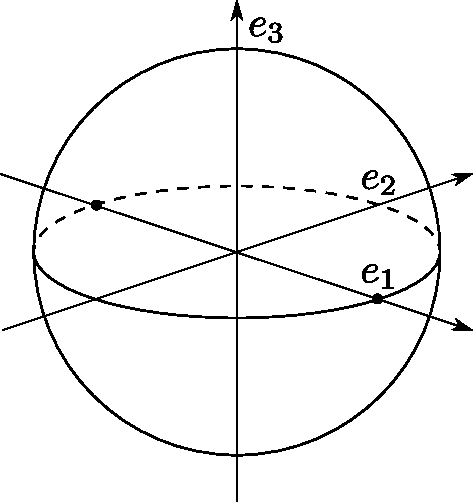
\includegraphics[width=2in]{905/Figures/15-sphere-CW-structure.pdf}
\end{center}

Now there are two $k$-cells for each $k$ with $0\leq k\leq n$, given by the
two hemispheres of $S^k$. For each $k$ there are two characteristic maps,
\[
u,\ell:D^k\to S^k 
\]
defining the upper and lower hemispheres:
\[
u(x)=(x,\sqrt{1-|x|^2})\,,\quad\ell(x)=(x,-\sqrt{1-|x|^2})\,.
\]
Note that if $|x|=1$ then $|u(x)|=|\ell(x)|=1$, so each characteristic map
restricts on the boundary to a map to $S^{k-1}$, and serves as an attaching 
map. This cell structure has the advantage that $S^{n-1}$ is a subcomplex 
of $S^n$. 

The case $n=\infty$ is allowed here. Then $\RR^\infty$ denotes the countably
infinite dimensional inner product space that is the topological union of the
leading subspaces $\RR^n$. The CW-complex $S^\infty$ is of finite type but
not finite dimensional. It has the following interesting property. We know that
$S^n$ is not contractible (because the identity map and a constant map have 
different behavior in homology), but: 
\begin{prop}
$S^\infty$ is contractible.
\end{prop}
\begin{proof}
This is an example of a ``swindle,'' making use of infinite dimensionality. 
Let $T:\RR^\infty\to\RR^\infty$ send $(x_1,x_2,\ldots)$ to 
$(0,x_1,x_2,\ldots)$. This sends $S^\infty$ to itself. The location of the 
leading nonzero entry is different for $x$ and $Tx$, so the line segment 
joining $x$ to $Tx$ doesn't pass through the origin. Therefore 
\[
x\mapsto\frac{tx+(1-t)Tx}{|tx+(1-t)Tx|} 
\]
provides a homotopy $1\simeq T$. On the other hand, $T$ is homotopic to the 
constant map with value $(1,0,0,\ldots)$, again by an affine homotopy. 
\end{proof}

This ``inefficient'' CW structure on $S^n$ has a second advantage: it's
{\em equivariant} with respect to the antipodal involution. This provides us
with a CW structure on the orbit space for this action. 

Recall that $\mathbf{RP}^k=S^k/\sim$ where $x\sim -x$. The quotient map
$\pi:S^k\to\mathbf{RP}^k$ is a double cover, identifying upper and lower 
hemispheres. The inclusion of one sphere in the next is compatible with
this equivalence relation, and gives us ``linear'' embeddings 
$\mathbf{RP}^{k-1}\subseteq\mathbf{RP}^k$. 
This suggests that
\[
\varnothing\subseteq\mathbf{RP}^0\subseteq\mathbf{RP}^1\subseteq\cdots
\subseteq\mathbf{RP}^n
\]
might serve as a CW filtration. Indeed, for each $k$,
\begin{equation*}
\xymatrix{
S^{k-1} \ar[r] \ar[d]^\pi & D^k \ar[d]^u \\
\mathbf{RP}^{k-1} \ar[r] & \mathbf{RP}^k 
}\end{equation*}
is a pushout: A line in $\RR^{k+1}$ either lies in $\RR^k$ or is determined 
by a unique point in the upper hemisphere of $S^k$.



